\chapter{Simple Controller} \label{chap:controllerPattern}
\section{Case Description}

The Simple Controller model showcases a simple design pattern for
connecting an existing CT plant model to a DE model. 
The overall model consists of three main blocks (see Figure~\ref{fig:20simmotor}),
\texttt{Controller}, \texttt{IO}, and \texttt{Plant}. The
\texttt{Controller} block houses the controller that calculates an
appropriate output for the motor. The \texttt{IO} block
resides between the \texttt{Controller} and the \texttt{Plant}, and
handles D/A and A/D conversion, scaling and quantization.

The plant represents a motor which drives a wheel (for example,
on a car) to achieve a desired target speed, with a closed feedback
loop. The controller computes a motor steering value, using the difference between the set point and the measured value (from the encoder). 
The motor applies torque to a rotating wheel, and an encoder monitors actual rotations and feeds this information back to the controller.  

There are two versions of the Simple Controller model provided, which can be
compared side-by-side (it is possible to switch between the two models
in 20-sim).  One version is entirely implemented as a CT model, with a
CT controller block to interact with the motor and an encoder.  
The second version is a \DESTECS co-model, which has a controller
implemented in VDM.  Because there are two versions of the model
provided, the Simple Controller may be of interest to those with a
background in CT modelling who want to see how to convert an existing
CT model to a \DESTECS co-model. The design pattern visible in the
co-model here is reused in many other, more complex \DESTECS co-models.

\begin{figure}[!ht]
\begin{subfigure}
\centering
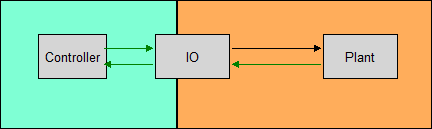
\includegraphics[width=0.5\linewidth]{controllerPattern/toplevel}
\end{subfigure}
\begin{subfigure}
\centering
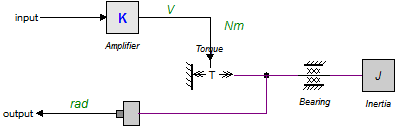
\includegraphics[width=0.45\linewidth]{controllerPattern/plant}
\end{subfigure}
\caption{The 20-sim top level model (left) and the plant (right)}
\label{fig:20simmotor}
\end{figure}

\section{Contract} The contract contains two variables of type
\keyw{real}. A monitored variable, \texttt{counts}, represents data
returned from the sensor monitoring the movement of the wheel, in the
form of a figure representing the number of radians rotated. A
controlled variable, \texttt{rev}, produces a output signal for the
motor actuator.

\section{Discrete-event} The DE model contains a
\texttt{Controller} class, which has the main thread of control.  The
\texttt{Control\-ler} instantiates abstract classes to represent the
actuator (\texttt{IActuatorReal}) and the sensor
(\texttt{ISensorReal}). At run-time concrete implementations of these
classes are provided by the \texttt{Actuator} class and the
\texttt{Sensor} class respectively. Designing a controller that
primarily handles abstract classes makes it easier to replace or alter
the concrete implementation at a later date if necessary.

The \texttt{Controller} is deployed onto a CPU running at 10MHz
by the \texttt{System} class.

\section{Continuous-time} There are two versions of the CT model
provided in 20-sim, one with all control implemented entirely in a CT
(20-sim) model, and one with all control implemented in VDM (i.e., a
\DESTECS co-model). Both models share the same plant, in which a power
signal, \emph{K}, is output to a motor, \emph{T}, which produces torque to rotate
a wheel, \emph{J}, modeling its inertia, whilst the bearing attached to the wheel models friction.

In the CT-only model the
\texttt{Controller} block houses the controller that calculates an
appropriate output for the motor. 

In the second model - a \DESTECS co-model - the
functionality previously implemented by the \texttt{Controller}
has now been moved into a VDM model in the \DESTECS tool, and so the second implementation of the 
\texttt{Controller} block, now takes responsibility for importing data to and exporting data
from the DE model. 

With two implementations available, the Simple Controller model
permits a modeller to experiment by locating different functionalities
in different parts of the model (for example, moving the controller
functionality from the CT model to the DE model) and comparing the
results. 

\section{Usage} 
The Simple Controller is a simple
example of a basic model. A good way to see how the model works
would be to run and compare the two versions (the CT-only and
the co-model). The CT-only model should be launched directly
from 20-sim. To do this, right click on the high-level \texttt{Controller} block in
20-sim, select \texttt{Edit Implementation}, and select
\texttt{CT}, and launch the model. 
Alternatively one can select \texttt{Destecs} here and
then launch the co-simulation from the \DESTECS tool.
